\chapter{Conception}


%% ------------------------------------------ %%
%%               ARCHITECTURE                 %%
%% ------------------------------------------ %%
\section{Architecture du système}\label{conception.architecture}

\todo{Description générale ?}

\subsection{Capture des images}
Cette section présente l'architecture du système de capture d'image du parking, nécessaire à ce projet. Une caméra IP sera choisie, qui sera connectée au réseau de la HEIG-VD de la manière décrite ici. La capture d'image a été pensée afin de permettre la connexion de multiple caméra.

Il faudra remarquer que les choix effectués ici non seulement influence la caméra qui sera choisie en section \ref{conception.techno.camera} \nameref{conception.techno.camera}, mais aussi, ces choix dépendent de celle-ci. Ainsi, ces deux travaux (choix de l'architecture de capture d'image et choix de la caméra) ont été réalisés en parallèle.

\todo{descritpion}

\subsubsection{Architecture logique}
%\nomenclature{VM}{machine virtuelle, pour \textit{Virtual Machine} en anglais}

La caméra réseau sera connectée au réseau local de la HEIG-VD. Elle aura donc une adresse IP, qu'il sera possible d'utiliser afin de dialoguer avec elle. Une machine virtuelle (abrégée \textit{VM}, pour \textit{Virtual Machine}) a été mise à disposition de ce projet. Située sur le réseau de l'école, elle permettra de récupérer ses images.

\begin{figure}[h]
    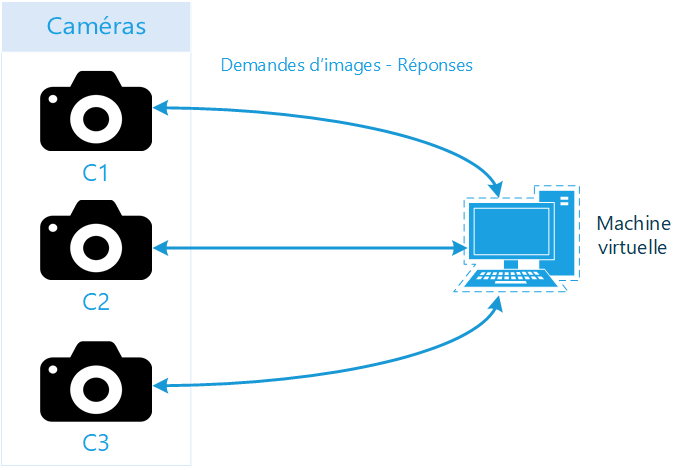
\includegraphics[width=150mm]{img/conception/logic_arch.png}
    \label{fig:capture_cameras}
    \centering
    \caption{Capture d'images de plusieurs caméras}
\end{figure}

La figure \ref{fig:capture_cameras} présente un protocole de demande-réponse sur \textit{HTTP} qui sera utilisé afin de récupérer des images à intervalles réguliers. On pourra la préciser ainsi:

\begin{enumerate}
    \item La \textit{VM} emmet une requête demandant l'image du parking à une caméra. 
    \item La caméra répond à la \textit{VM} avec ladite image.
\end{enumerate}

Les requêtes et réponses précitées sont fortement dépendantes de la caméra choisie. Ainsi, les détails d'implémentation pourront être trouvés en section \ref{realisation.capture} \nameref{realisation.capture}.


\subsubsection{Architecture physique}
\paragraph{Connexion de la caméra}\label{conception.architecture.physique.camera}
\todo{Schéma des différentes connexions possible + choix}

%\paragraph{Réseau} % pas très important ?
%\todo{Schéma réseau physique}
\todo{Pas très important schéma réseau physique ?}


\todo{Architecture choisie : sur le toit, construction d'une salle en cours --> panneau solaire}

%% ------------------------------------------ %%
%%           CHOIX TECHNOLOGIQUES             %%
%% ------------------------------------------ %%

\section{Choix technologiques}

\subsection{Caméra réseau}\label{conception.techno.camera}
Une caméra réseau fournissant des images de qualités, et ce dans un prix raisonable, est nécessaire dans ce projet afin de capturer des images. Celle-ci sera utilisée principalement dans 2 buts, précisés ci-après.

\paragraph{Entrainement du modèle}
Dans un premier temps, il s'agit d'entrainer le modèle à partir des images fournies par la caméra. Pour ce faire, il doit être possible de capturer des photos à intervalles réguliers. Ces images seront ensuite annotées, puis utilisées pour entrainer le modèle du réseau de neurones à convolutions. 

\paragraph{Utilisation du modèle}
Une fois le modèle définit, le but de ce projet est de l'utiliser afin de détecter le nombre de voiture présentes courant sur le parking. Ainsi, dans un second temps, la caméra doit pouvoir fournir des images du parking "en direct", dans le but d'obtenir un état courant du parking. Il faut noter qu'ici, la notion "en direct" signifie "relativement court", soit de l'ordre de la minute. En effet, en tant qu'utilisateur, obtenir le taux d'occupation du parking à la minute près semble suffisant. Bien entendu, un intervalle plus court entre chaque prise, ou un flux vidéo, est un plus.

\subsubsection{Contraintes}\label{conception.techno.camera.contraintes}
Installer une caméra sur le toit de la HEIG-VD a pour conséquence que certaines contraintes, tant d'ordre techniques qu'organisationnelles, doivent être respectées. Celles-ci sont décrites dans cette section.

\paragraph{Capture de photo}
La caméra devra au minimum permettre la capture de photos à intervalles réguliers d'une façon ou d'une autre. L'intervalle minimum de capture est de l'ordre de la minute, afin de pouvoir obtenir l'état courant du parking filmé . La capture de vidéos n'est pas nécessaire. On notera que si celle-ci ne fournit malheureusement que la fonctionnalité de capture vidéo, il serait tout de même possible d'en extraire des images utilisables. 

\paragraph{Usage extérieur}
La caméra doit être prévue pour un usage extérieur, avec une protection contre les intempéries (pluie, neige, froid, chaud, etc.)

\paragraph{Connexion réseau}
En lien avec le paragraphe précédent, la caméra doit nécessairement avoir une interface Wifi permettant de se connecter au réseau de l'école. Une connexion par Ethernet n'est pas envisageable.

\paragraph{Caméra auto-alimentée}
Comme vu en section \ref{conception.architecture.physique.camera}, la caméra doit être auto-alimentée et non cablée. Ainsi, une combinaison de batteries et de panneaux solaires semble être idéal. On peut noter que l'utilisation de batteries uniquement est envisageable dans le cadre d'un prototypage, mais ce uniquement si le remplacement de celles-ci doit être effectué à intervalles relativement éloignés, de l'ordre de la semaine.

\paragraph{Résolution d'image}
Dans le but d'obtenir des images de qualités suffisantes, la résolution de l'image capturées devra nécessairement être d'au minimum 1280x720 pixels.

\subsubsection{Critères}
Plusieurs critères, ont été définis. Chacune des caméras retenues seront notées selon ceux-ci. On les trouvera ci-après, où leur pondération sont indiqués entre crochets ([]). Une pondération élevée signifie une plus grande importance de ce critère.

\paragraph{Qualité d'image [1]}
La caméra doit avoir une bonne qualité d'image. On jugera:
\begin{itemize}
    \item La résolutions de l'image. Celle-ci doit être d'au minimum 1280x720 pixels.
    \item La qualité de l'image (si possible).
\end{itemize}

\paragraph{Fonctionnalités réseaux [2]}
La caméra doit pouvoir fournir des images via le réseau et il doit être possible d'en récupérer à intervalles réguliers. Pour ce faire, on pensera à des protocoles comme les suivants: 
\begin{description}
    \item[ONVIF (Open Network Video Interface Forum)] Standard industriel ouvert permettant de contrôler, configurer et communiquer avec des caméras de sécurité IP. Permet notamment la lecture de flux vidéo en temps réel et la capture de photos \autocite{wiki:onvif}
    \item[RTSP (Real Time Streaming Protocol)] Développé par RealNetworks, Netscape et Clumbia UNiversity, protocole de communication permettant de lire en temps réel un flux vidéo. \autocite{wiki:RTSP}
    \item[Requêtes HTTP] Il pourrait être possible de capturer et de récupérer à la demande une photo à l'aide de requêtes HTTP.
    \item[Flux sur HTTP] Permet la lecture de flux vidéo sur HTTP en s'appuyant sur des formats tel que MPEG-4.
    \item[Interface Web HTTP] Permet la configuration de la caméra IP via un serveur Web qu'elle expose. 
    \item[FTP] La caméra peut exposer un serveur FTP contenant les photos capturées. Elle pourrait aussi téléverser des photos capturées sur un serveur FTP distant.
On notera avant tout sur la facilité d'utilisation des différents protocoles.
\end{description}

\paragraph{Fonctionnement auto-alimenté [4]}
La caméra doit être auto-alimentée et non cablée. Comme critères, on pensera donc à:
\begin{itemize}
    \item La durée de vie de la caméra en fonctionnement auto-alimenté. Idéalement, la caméra ne devrait nécessiter aucune intervention humaine.
    \item La portée du Wifi. La puissance du signal doit être assez forte afin de pouvoir capter les bornes Wifi de l'école depuis le toit de la HEIG-VD. Il est important de noter que ce critère peut être difficilement évalué avant l'achat de la caméra.
\end{itemize}

\paragraph{Capture de photo [2]}
La caméra doit être capable de fournir un moyen pour capturer des photos à intervalles réguliers, de l'ordre de la minute. Pour ce faire, la caméra peut fournir un système de capture de photos automatique, ce qui est un plus. On évaluera donc les moyens fournis par la caméra permettant ces captures.

\paragraph{Angle de vue [2]}
L'angle de vue de la caméra doit être suffisamment grand afin d'obtenir une image du parking dans son ensemble. Il peut être suffisant à partir de 40°, de par la hauteur à laquelle elle sera placée. Cependant, un angle de 90° semble plus satisfaisant. Ces angles ont été définis à l'aide des informations fournies par \url{videosurveillance-boutique.fr} \autocite{cam:securite_info}.

\paragraph{Vision de nuit [1]}
Idéalement, la caméra devrait pouvoir fournir une vision de nuit afin de pouvoir capturer des images de parking par toute heure. On pensera notamment aux matinées et aux soirées d'hiver, où les véhicules arrivent et partent alors que la luminosité est encore très faible. Cependant, dans le cadre de ce TB, cette fonctionnalité n'est pas strictement nécessaire.

\paragraph{Facilité d'installation [1]}
La facilité d'installation de la caméra sera prise en compte. On pensera aux dimensions de celle-ci, à son poids, au nombre de ses composants (par exemple, est-il nécessaire d'installer une batterie en plus de la caméra, ou est-elle incorporée à celle-ci?), ou encore aux accessoires fournis pour son installation. 

\paragraph{Prix [4]} Bien évidemment, le prix doit entrer en ligne de compte. 100.- CHF sera indiqué comme prix maximum afin d'obtenir la meilleure note. A partir de 500.- CHF, on évaluera ce prix comme étant mauvais.

\subsubsection{Caméras disponibles et évaluation}
Bien que la surveillance n'est pas un but de ce TB, les caméras de sécurités semblent être les plus adaptées. En effet, elles fournissent généralement des fonctionnalités de capture de photos, de connexion réseau, de vision de nuit, possèdent un angle de vue suffisant et sont souvent résistantes à un environnement extérieur. De plus, elles sont spécialement concues pour un usage qui s'apparente à celui qui de ce TB, et sont donc adaptées à la prise d'images de parking.

L'achat distinct d'une caméra, de panneaux solaires et de batteries est envisageable. Néanmoins, dans un premier temps, seuls des kits complets (caméra, batteries, panneaux solaires) ont été analysés. En effet, l'installation et le choix des différents composants nécessaires à un système solaire complet semble difficile lorsqu'on est pas du domaine, et des problèmes d'interopérabilité pourraient survenir. Ceci reste cependant une solution viable si aucun kit ne correspond aux contraintes définies.

De part les contraintes très spécifiques précisées jusqu'ici, le nombre de caméras les satisfaisant toutes sont peu nombreuses. On trouvera ci-après les kits complets solaires auto-suffisants qui ont été évalués. Il faut aussi noter que seules les caméras les plus appropriées sont indiquées ici.

\paragraph{\textbf{Electrosun} -- Caméra-surveillance-solaire}
\textit{Electrosun} est une entreprise de domotique solaire française. Entre autres, un kit solaire de caméra complet est mis en vente. \autocite{cam:electrosun_site}

\begin{figure}[h]
    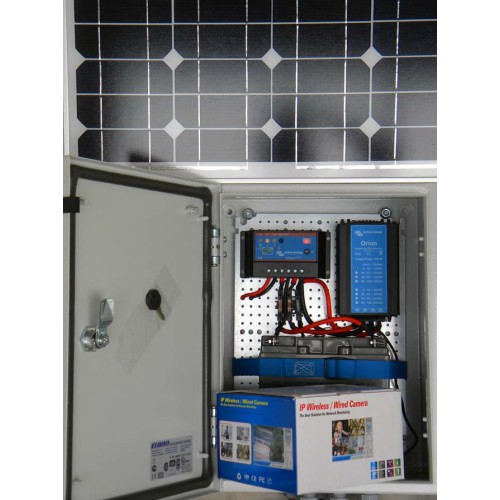
\includegraphics[width=50mm]{img/conception/electrosun_cam.jpg}
    \centering
    \captionsource{\textbf{Electrosun} Caméra de surveillance solaire}{\autocite{cam:electrosun_site}}
\end{figure}

Bien qu'elle satisfasse la plupart des contraintes, elle n'a pas été retenue pour l'évaluation. En effet, la résolution des images capturées n'est que de 640x480 pixels, ce qui n'est pas suffisant.

\paragraph{\textbf{Reolink} -- Argus 2}
L'entreprise \textit{Reolink} développe des caméras 100\% sans fil, avec batteries rechargeables et panneaux solaires. Elle est auto-suffisante.\autocite{cam:argus2}

\begin{figure}[h]
    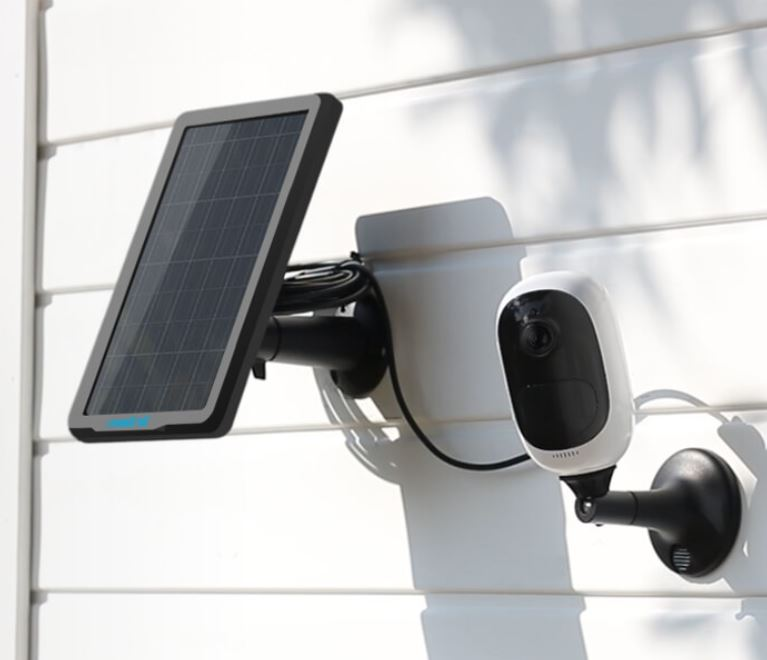
\includegraphics[width=50mm]{img/conception/argus2_cam.jpg}
    \centering
    \captionsource{\textbf{Reolink} Argus 2}{\autocite{cam:argus2}}
\end{figure}

Elle permet de capturer des photos FullHD (1920x1080 pixels), possède une fonction de vision de nuit ou encore, l'utilisation en extérieur est possible. Cependant, cette caméra n'a elle non plus pas pu être prise en considération. En effet, elle a été pensée pour un usage privé, et bien que la caméra puisse être connectée à un réseau Wifi, l'accès à celle-ci n'est possible qu'à l'aide d'une application smartphone (tel que décrit dans les spécifications disponibles sur le site officiel \url{https://reolink.com/product/argus-2}\autocite{cam:argus2}). Récupérer des photographies à intervalles réguliers semble donc difficilement réalisable.

\paragraph{\textbf{Wanscam} -- HW0029-3}

\textit{Wanscam} est une entreprise chinoise spécialisées dans la production de caméra réseau. Plusieurs versions de son modèle \textit{HW0029} sont disponibles. Ici est présenté le modèle \textit{HW0029-3}. \autocite{cam:wan3}

\begin{figure}[h]
    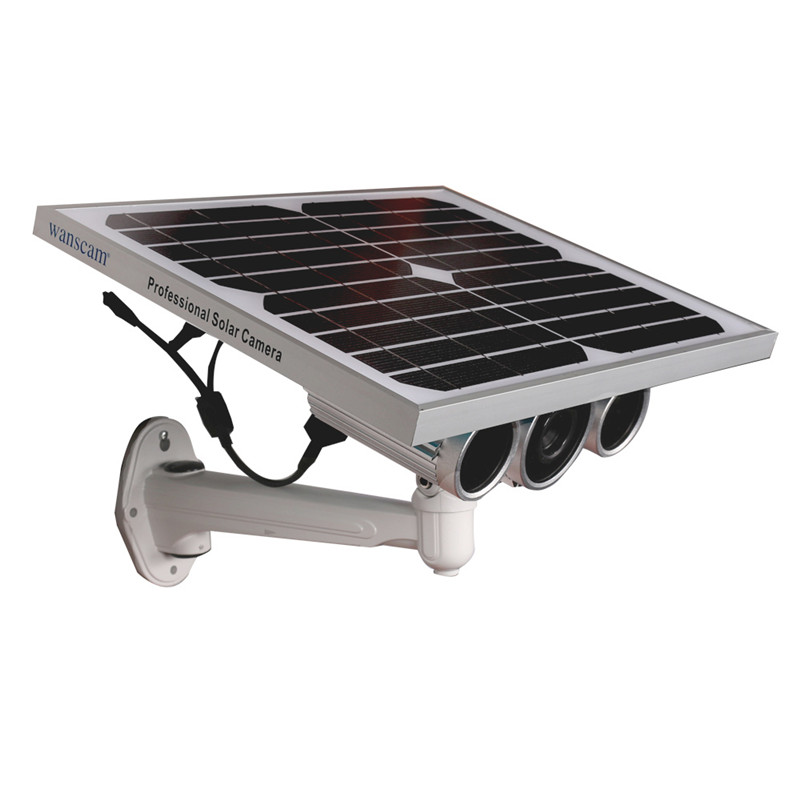
\includegraphics[width=50mm]{img/conception/wan3_cam.jpg}
    \centering
    \captionsource{\textbf{Wanscam} HW0029-3}{\autocite{cam:wan3}}
\end{figure}

Cette caméra satisfait toutes les contraintes définies en section \ref{conception.techno.camera.contraintes}. On trouvera en table \ref{tab:HW0029-3} ses principales caractéristiques.\footnote{Tirées des spécifications officielles \autocite{cam:wan3} et d'un test indépendant \autocite{cam:wan3-test}}

\begin{table}[H]
    \centering
    \caption{Caractéristiques de la caméra \textbf{Wanscam} \textit{HW0029-3}}
    \label{tab:HW0029-3}
    \begin{tabular}{@{}ll@{}}
    \toprule
    Caractéristique        & Valeurs                                                                                                                                                                                                                                                                                     \\ \midrule
    Image                  & 1280 x 720, 25fps, compression H.264                                                                                                                                                                                                                                                        \\ [0.8ex]
    Angle de vue           & 40°                                                                                                                                                                                                                                                                                         \\ [0.8ex]
    Vision nocture         & Visibilité jusqu'à 15 mètres                                                                                                                                                                                                                                                                \\ [0.8ex]
    Réseau                 & RJ45, WiFi 802.11 b/g/n                                                                                                                                                                                                                                                                     \\ [0.8ex]
    Auto-alimentation      & \begin{tabular}[c]{@{}l@{}}2 batteries de 12A et panneau solaire. \\ Sans soleil: 48h d'utilisation. \\ Faible température (\textless 26°) des rayons de soleil: 7 jours d'utilisations. \\ Grande température (\textgreater 33°) des rayons de soleil: fonctionnement continu\end{tabular} \\ [0.8ex]
    Stockage               & Carte MicroSD de 16Gb incluse, support jusqu'à 128Gb                                                                                                                                                                                                                                        \\ [0.8ex]
    Détection de mouvement & Oui                                                                                                                                                                                                                                                                                         \\ [0.8ex]
    Accès aux images       & Flux HTTP, ONVIF, RTSP, requêtes HTTP                                                                                                                                                                                                                                                       \\ [0.8ex]
    Dimensions et poids    & 370x290x110 mm, 2.7 kg                                                                                                                                                                                                                                                                      \\ \bottomrule
    \end{tabular}
\end{table}

On notera que le panneau solaire est fixé sur la caméra. Ainsi, dans le but de garder une exposition au soleil suffisante, l'angle de la caméra ne doit pas être trop élevé. Il y a donc certaines contraintes à l'installation de celle-ci.

Concernant la capture d'image, la caméra fournit des \textit{endpoints HTTP} (dont une liste peut être trouvée sur le site \url{tutoriels.domotique-store.fr}\autocite{cam:wan3-url}) permettant de récupérer l'image actuelle. Il est donc facile d'imaginer un simple agent qui, à intervalle régulier, demandera à la caméra une image, et l'enregistrera en local.

Les caméras \textbf{Wanscam} ne sont pas des plus faciles à trouver dans le commerce. Elles sont principalement disponibles sur \url{aliexpress.com}. Le modèle \textit{HW0029-3} peut être trouvé à partir de 170CHF (en date du 09.03.2018, \url{aliexpress.com}).

La grille d'évaluation \ref{cam:wan3_eval} a pu être remplie à l'aide de ces spécifications.

\begin{table}[H]
    \centering
    \caption{Evaluation de la caméra \textbf{Wanscam} \textit{HW0029-3}}
    \label{cam:wan3_eval}
    \begin{tabular}{@{}llp{8cm}@{}}
        \toprule
        Critère                              & Note (de 1 à 5) & Remarque                                                                                                                                                                   \\ \midrule
        Qualité d'image              & 3 [1]               & La qualité d'image semble suffisante selon les tests effectué par \url{lesbonstuyauxgeeks.fr}\autocite{cam:wan3-test}. La résolution est de 1280x720 pixels, ce qui est suffisant. \\ [0.8ex]
        Fonctionnalités réseaux      & 5 [2]              & La caméra offre notamment un endpoint HTTP sur lequel récupérer les images.                                                                                                \\ [0.8ex]
        Fonctionnement auto-alimenté & 4 [4]              & La caméra est totalement auto-suffisante s'il y a assez de soleil. On notera cependant le panneau solaire fixe qui peut nuire à l'exposition du soleil. Elle supporte le Wifi 802.11n: à première vue, le signal semble suffisant.                   \\ [0.8ex]
        Capture de photo             & 5 [2]              & Il est facile de récupérer des images sur cette caméra. Elle offre en plus un système de capture de photos à intervalles réguliers automatique. Elle offre aussi la possibilité de récupérer un flux vidéo.                            \\ [0.8ex]
        Angle de vue                 & 1 [2]              & Un angle de vue de 40° semble tout juste suffisant.                                                                                                                        \\ [0.8ex]
        Vision de nuit               & 2 [1]               & Elle fournit une vision nocturne à 15m. Il est cependant possible d'ajouter des LEDs infrarouges supplémentaires afin d'obtenir une meilleure vision de nuit\autocite{cam:wan3-url}. \\ [0.8ex]
        Facilité d'installation      & 3 [1]              & La caméra mesure jusqu'à 37 cm, ce qui nuit à sa facilité d'installation. De plus, le panneau solaire est fixe, ce qui contraint la position et l'angle de la caméra.      \\ [0.8ex]
        Prix                         & 4 [4]              & A partir d'environ 170.- CHF \\ \midrule
        && \textbf{Note finale: 3.6/5} \\ \bottomrule
    \end{tabular}
\end{table}

\paragraph{\textbf{Wanscam} -- HW0029-5}
Le modèle \textit{HW0029-3} de \textbf{Wanscam} est la nouvelle version du modèle \textit{HW0029-3} décrit précédemment. Elle possède la plupart des mêmes caractéristiques, mais propose une meilleure résolution (1920x1080), des batteries à plus grande capacité, un meilleur champ de vision, ou encore, une vision de nuit accrue jusqu'à 100m. Son prix est cependant plus élevé que la caméra \textit{HW0029-3}. Les caractéristiques indiquées dans ce rapport proviennent du site officiel \url{wanscam.com}\autocite{cam:wan5}.

\begin{figure}[h]
    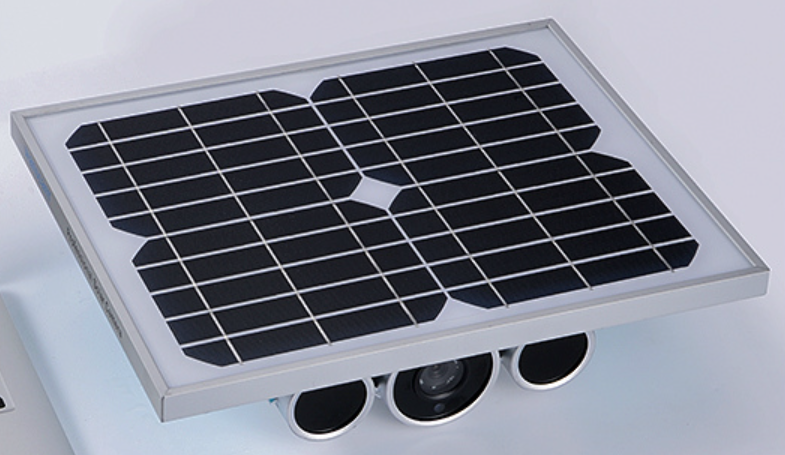
\includegraphics[width=50mm]{img/conception/wan5_cam.png}
    \centering
    \captionsource{\textbf{Wanscam} HW0029-5}{\autocite{cam:wan5}}
\end{figure}

\begin{table}[H]
    \centering
    \caption{Caractéristiques de la caméra \textbf{Wanscam} \textit{HW0029-5}}
    \label{tab:HW0029-5}
    \begin{tabular}{@{}ll@{}}
    \toprule
    Caractéristique        & Valeurs                                                                                                                                                                                                                                                                                     \\ \midrule
    Image                  & 1920 x 1080, 25-30fps, compression H.264                                                                                                                                                                                                                                                        \\ [0.8ex]
    Angle de vue           & 80°                                                                                                                                                                                                                                                                                         \\ [0.8ex]
    Vision nocture         & Visibilité jusqu'à 100 mètres                                                                                                                                                                                                                                                                \\ [0.8ex]
    Réseau                 & RJ45 100Mbps, WiFi 802.11 b/g/n                                                                                                                                                                                                                                                                     \\ [0.8ex]
    Auto-alimentation      & \begin{tabular}[c]{@{}l@{}}2 batteries de 12A et panneau solaire. \\ Sans soleil: 54h d'utilisation. \end{tabular} \\
    Stockage               & Carte MicroSD de 16Gb incluse, support jusqu'à 128Gb                                                                                                                                                                                                                                        \\ [0.8ex]
    Détection de mouvement & Oui                                                                                                                                                                                                                                                                                         \\ [0.8ex]
    Accès aux images       & Flux HTTP, ONVIF, RTSP, requêtes HTTP                                                                                                                                                                                                                                                       \\ [0.8ex]
    Dimensions et poids    & 370x286x960 mm, 4.3 kg                                                                                                                                                                                                                                                                      \\ \bottomrule
    \end{tabular}
\end{table}

Il faudra noter que cette caméra est plus lourde, bien que plus petite, que le précédent modèle. 

De ces caractéristiques, il a été possible d'évaluer cette caméra dans la grille d'évaluation \ref{cam:wan5_eval} 

\begin{table}[H]
    \centering
    \caption{Evaluation de la caméra \textbf{Wanscam} \textit{HW0029-5}}
    \label{cam:wan5_eval}
    \begin{tabular}{@{}llp{8cm}@{}}
        \toprule
        Critère                      & Note (de 1 à 5) & Remarque                                           \\ \midrule
        Qualité d'image              & 4 {[}1{]}       & La qualité de l'image est meilleure que le modèle précédent, avec une résolution de 1920x1080 pixel.                                                              \\ [0.8ex]
        Fonctionnalités réseaux      & 5 {[}2{]}       & La caméra offre notamment un endpoint HTTP sur lequel récupérer les images.                                                                                       \\ [0.8ex]
        Fonctionnement auto-alimenté & 4 {[}4{]}       & De la même manière que le modèle précédent, la caméra est totalement auto-suffisante s'il y a assez de soleil. Sans soleil, elle est auto-suffisante jusqu'à 54h. Elle support la norme Wifi 802.11n \\ [0.8ex]
        Capture de photo             & 5 {[}2{]}       & Il est facile de récupérer des images sur cette caméra. De plus, elle offre un système de capture de photos à intervalles réguliers automatiques. Elle offre aussi la possibilité de récupérer un flux vidéo.                  \\ [0.8ex]
        Angle de vue                 & 4 {[}2{]}       & Un angle de vue de 80° semble être approprié pour ce projet. Un angle supérieur n'aurait pas été superflu.                                                        \\ [0.8ex]
        Vision de nuit               & 5 {[}1{]}       & Elle fournit une vision nocturne à 100m.                                                                                                                          \\ [0.8ex]
        Facilité d'installation      & 3 {[}1{]}       & Tout comme le modèle HW0029-3, la caméra n'est pas des plus petites, mesurant jusqu'à 37 cm. Le panneau solaire est fixé à la caméra.                             \\ [0.8ex]
        Prix                         & 3 {[}4{]}       & A partir d'environ 230.- CHF   \\ \midrule
        && \textbf{Note finale: 4.0/5} \\ \bottomrule
    \end{tabular}
\end{table}

\subparagraph{Remarque} Le modèle \textbf{Wanscam} \textit{HW0029-4} (ainsi que sa version améliorée \textit{HW0029-6}) n'a pas été pris en compte. En effet, il fourni en plus un système de puce 4G afin de pouvoir connecter la caméra à un réseau mobile. En conséquence, le prix est trop élevé, dépassant les 400.- CHF.

\paragraph{\textbf{Visortech} -- Caméra Solaire IP}
Cette caméra satisfait toutes les contraintes définies dans la section \ref{conception.techno.camera.contraintes} \nameref{conception.techno.camera.contraintes}. Ses caractéristiques principales sont décrites à la table \ref{tab:visortech_spec}. Il a été possible de remarquer que la caméra décrite ici est disponible sous différents noms, comme \textit{IdealSmartCam}.

\begin{figure}[h]
    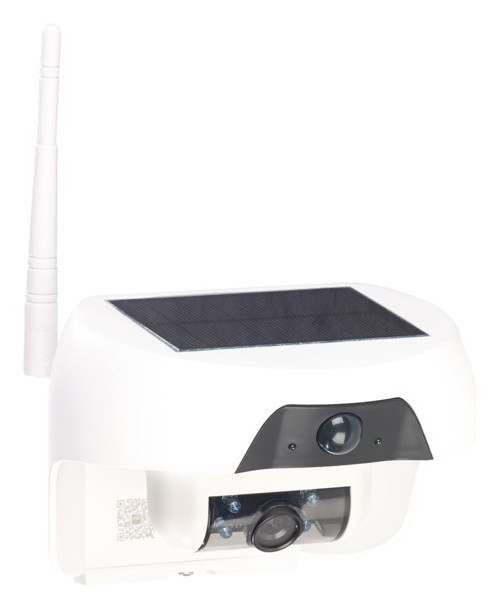
\includegraphics[width=50mm]{img/conception/visortech_cam.jpg}
    \centering
    \captionsource{Caméra Visortech}{\autocite{cam:visortech}}
\end{figure}

On notera le peu d'information disponible concernant les spécifications de cette caméra. Par exemple, il est difficile de connaitre les méthodes disponibles afin de pouvoir récupérer des images depuis le réseau local, tant et si bien que cela soit possible. On notera que le vendeur a été contacté, sans réponse de sa part.

\begin{table}[H]
    \centering
    \caption{Caractéristiques de la caméra \textit{Visortech}}
    \label{tab:visortech_spec}
    \begin{tabular}{@{}ll@{}}
    \toprule
    Caractéristique        & Valeurs                                                          \\ \midrule
    Image                  & 1280 x 720, compression H.264. Prise de vue en continu possible. \\ [0.8ex]
    Angle de vue           & 90°                                                              \\ [0.8ex]
    Vision nocture         & Visibilité jusqu'à 5 mètres                                      \\ [0.8ex]
    Réseau                 & Wifi 802.11 b/g/n                                                \\ [0.8ex]
    Auto-alimentation      & Panneau solaire intégré de 0.8 Watt, jusqu'à 5 jours sans soleil. Auto-suffisante.     \\ [0.8ex]
    Détection de mouvement & Oui                                                              \\ [0.8ex]
    Dimensions et poids    & 161x155x108 mm, 0.8 kg                                            \\  [0.8ex]\bottomrule
    \end{tabular}
\end{table}

Malgré le manque d'information, cette caméra a tout de même été évaluée. Il sera de ce fait possible de savoir si elle peut être un choix viable, ou non. La grille d'évaluation correspondante peut être trouvée en table \ref{tab:visortech_eval}

\begin{table}[H]
    \centering
    \caption{Evaluation de la caméra \textit{Visortech}}
    \label{tab:visortech_eval}
    \begin{tabular}{@{}llp{8cm}@{}}
        \toprule
        Critère                      & Note (de 1 à 5) & Remarque                          \\ \midrule
        Qualité d'image              & 3 {[}1{]}       & Sa résolution est de 1280x720 pixel.                                                                                                  \\ [0.8ex]
        Fonctionnalités réseaux      & 2 {[}2{]}       & Accès via smartphone possible, peu d'informations concernant les protocoles réseaux disponibles.                                      \\ [0.8ex]
        Fonctionnement auto-alimenté & 3 {[}4{]}       & Devrait être auto-suffisante. Cependant, informations peu claires si prises d'images en continu. Accepte la norme Wifi 802.11n. \\ [0.8ex]
        Capture de photo             & 3 {[}2{]}       & Permet l'accès au flux vidéo en direct. Peu d'informations sur les protocoles disponibles.                                            \\ [0.8ex]
        Angle de vue                 & 5 {[}2{]}       & Angle de vue de 90°. Meilleur champ de vision parmi les caméras évaluées.                                                              \\ [0.8ex]
        Vision de nuit               & 2 {[}1{]}       & Elle fournit une vision nocturne à 5m.                                                                                                \\ [0.8ex]
        Facilité d'installation      & 3 {[}1{]}       & La caméra est relativement petite, et ne pèse que 850g. On notera l'absence de pied: une fixation à un mur semble nécessaire.         \\ [0.8ex]
        Prix                         & 3 {[}4{]}       & A partir d'environ 220.- CHF                                                                                                          \\ [0.8ex]
                                    &                 & \textbf{Note finale: 3.1/5} \\ \bottomrule
    \end{tabular}
\end{table}

\subsubsection{Choix final}

La caméra \textit{Visortech} arrive dernière du classement, avec une note de 3.1. Ceci est avant tout du au manque d'information sur les protocoles utilisables afin de récupérer via le réseau des images. Elle n'a donc pas été retenue.

\begin{table}[!h]
    \centering
    \caption{Caméras - Synthèse des résultats}
    \label{cam:synthese}
    \begin{tabular}{@{}lll@{}}
    \toprule
      & Caméra           & Note \\ \midrule
    \textbf{1} & Wanscam HW0029-5 & 4.0  \\
    \textbf{2} & Wanscam HW0029-3 & 3.6  \\
    \textbf{3} & Visortech        & 3.1  \\ \bottomrule
    \end{tabular}
\end{table}

Les deux versions de la caméra \textit{HW0029} de \textbf{Wanscam} montrent des résultats proches. Elles sont avant tout distinguable par leur qualité d'image, leur vision de nuit, leur durée de fonctionnement sur batterie et leur angle de vue, où toutes ses caractéristiques sont améliorées sur le nouveau modèle (\textit{HW0029-5}). Ainsi, seul le rapport qualité/prix peut faire pencher la balance d'un côté ou d'un autre. Avec un peu de recherche, la version \textit{HW0029-5} a été trouvée à 187.50€ sur \url{aliexpress.com}\autocite{cam:wan5-buy} (frais de livraison inclu), soit 225.- CHF (1.17CHF/€ en date du 13 mars 2018\autocite{util:cours}, arrondi au dizième supérieur, soit 1.20 CHF/€). 

Au prix indiqué plus haut, et vis-à-vis du classement présenté en table \ref{cam:synthese}, la caméra \textbf{Wanscam} \textit{HW0029-5} a été choisie pour la capture d'image que demande ce projet.

































\section{Limitations}